\labeledsection{Mathematical Structures}{sec:math_structure}
\definition{Mathematical Structure}{
A mathematical structure combines multiple \linkterm{mathematical objects}{math_object} (the components) into a new \linkterm{object}{math_object}. The components usually have names by which they can be referenced. Given a \linkterm{definition}{definitions} of a mathematical structure $S$, we say that any \linkterm{object}{math_object} that conforms to that is an instance of $S$.
}{def:math_structure}
\textbf{Example: }A graph $G = \tuple{V,E}$ is a \linkterm{mathematical structure}{def:math_structure} where the components are: $V$ (the \linkterm{set}{def:set} of vertices) and $E$ (the \linkterm{set}{def:set} of edges). A graph $G$ where $V = \set{1,2,3}$ and $E=\set{(1,2),(2,3)}$ is one instance of a graph.

\definition{Structure Signature}{
A structure signature combines the components, their types, and accessor names of a \linkterm{mathematical structure}{def:math_structure} in a tabular overview.
}{structure_signature}
\textbf{Example: }

\[
\left\langle
\begin{array}{lll}
V & \text{Set} & \text{vertices (nodes)} \\
E & \setbuilder{(u,v)}{u,v \in V} & \text{edges} \\
\end{array}
\right\rangle
\]

\commandnote{
Most programming languages have some way of creating \textit{"named structures"} and referencing components is usually done via \textit{"dot notation"} (e.g. \texttt{person.name}).
}

\definition{Group}{
A group is a \linkterm{mathematical structure}{def:math_structure} $\tuple{G, \circ, e, \inverse{.}}$ that consists of:
\begin{itemize}
    \item a base \linkterm{set}{def:set} $G$ of \linkterm{objects}{math_object},
    \item an operation $\circ : \cartprod{G,G} \to G$, such that $\forall a,b \in G. a \circ b \in G$ and $\forall a,b,c \in G. (a \circ b) \circ c = a \circ (b \circ c)$,
    \item a unit $e \in G$, such that $\forall a \in G. e \circ a = a \circ e = a$, and
    \item the \linkterm{inverse function}{inverse_function} $.^{-1} : G \to G$, such that $\forall a \in G. a \circ \inverse{a} = \inverse{a} \circ a = e$
\end{itemize}
}{group}
An example of a \linkterm{group}{group} is the \linkterm{set}{def:set} $G = \mathbb{Z}$, with the operation $\func{+}{\cartprod{\mathbb{Z},\mathbb{Z}}}{\mathbb{Z}}$; then $e = 0$ and $\inverse{.}$ is $\lambda x \in \mathbb{Z}. -x$. We write it as $\tuple{\mathbb{Z}, +, 0, -}$.

\textbf{Question: }can we do the same for multiplication where $e = 1$? If we think about it, we would be stuck on finding the $\inverse{.}$ component of the group. What can we always multiply with any integer and get $e=1$ back? Take for example $1$, we can multiply it with $\frac{1}{1}$ (great!). Take $-1$, we can multiply it with $\frac{1}{-1}$ (also great!). But take any other integer, e.g. $2$, we must multiply it with $\frac{1}{2}$ to get $1$ back, however, $\frac{1}{2} \notin \mathbb{Z}$, it is however $\in \mathbb{Q}$! Moreover, $0$ never has a multiplicative inverse in any field! The multiplicative group would only make sense iff $G = \mathbb{Q} \setminus \set{0}$. We write that as $\tuple{\mathbb{Q} \setminus \set{0}, * , 1, a \mapsto \frac{1}{a}}$.

\textbf{But }we need some \linkterm{multiplication}{multiplication} \linkterm{structure}{def:math_structure} that works for $\mathbb{Z}$!

\definition{Monoid}{
A monoid is a \linkterm{mathematical structure}{def:math_structure} $\tuple{M, \circ , e}$ that consists of:
\begin{itemize}
    \item A base set $M$ of \linkterm{objects}{math_object},
    \item An operation $\circ : M \times M \to M$, such that for all $a,b \in M$, we have $a \circ b \in M$ (closure),
    \item Associativity: for all $a,b,c \in M$, $(a \circ b) \circ c = a \circ (b \circ c)$, and
    \item A unit element $e \in M$, such that for all $a \in M. e \circ a = a \circ e = a$.
\end{itemize}
}{monoid}

Hence, the \linkterm{mathematical structure}{def:math_structure} $\tuple{\mathbb{Z}, * , 1}$ is a \linkterm{monoid}{monoid} (a \linkterm{group}{group} missing an \linkterm{inverse function}{inverse_function}).


We saw that $\tuple{\mathbb{Z}, +, 0, -}$ is a \linkterm{group}{group} under addition. And $\tuple{\mathbb{Z}, *, 1}$ is a \linkterm{monoid}{monoid} under multiplication. Now, we want to do everyday \linkterm{arithmetics}{arithmetic} with integers; we want expressions where we have additions and \linkterm{multiplication}{multiplication} (e.g. $a * (b + c)$) which evaluates to $(a * b) + (a * c)$.

For that, we need a \linkterm{mathematical structure}{def:math_structure} where both addition and \linkterm{multiplication}{multiplication} live together.

\definition{Ring}{
A ring is a \linkterm{mathematical structure}{def:math_structure} $\tuple{R, + , 0 , - , * , 1}$ consisting of:
\begin{itemize}
    \item A base \linkterm{set}{def:set} $R$.
    \item An addition operation $+: R \times R \to R$ such that $\tuple{R,+,0,-}$ is a \linkterm{group}{group} (called abelian \linkterm{group}{group}).
    \item A multiplication operation $*:R \times R \to R$ such that $\tuple{R, * , 1}$ is a \linkterm{monoid}{monoid}.
    \item Distributivity: for all $a,b,c \in R, a * (b+c) = (a*b) + (a*c), (a+b)*c = (a*c) + (b*c)$
\end{itemize}
}{ring}

Hence, mixing components from the \linkterm{group}{group} $\tuple{\mathbb{Z}, +, 0, -}$ and the \linkterm{monoid}{monoid} $\tuple{\mathbb{Z}, * , 1}$ leaves us with a \linkterm{ring}{ring} $\tuple{\mathbb{Z}, +, 0, -, *, 1}$


\definition{Magma}{
A magma is a \linkterm{mathematical structure}{def:math_structure} $\tuple{M, \circ}$ consisting of:
\begin{itemize}
    \item A base \linkterm{set}{def:set} $M$, and 
    \item A binary operation $\circ: M \times M \to M$.
\end{itemize}
}{magma}
\textbf{Example: } $\tuple{\mathbb{Z}, -}$ (integers under subtraction). $\tuple{\mathbb{N}, +}$ (natural numbres under addition)

\definition{Semigroup}{
A semigroup (\linkterm{magma}{magma} with associativity) is a \linkterm{mathematical structure}{def:math_structure} $\tuple{S, \circ}$ consisting of:
\begin{itemize}
    \item A base \linkterm{set}{def:set} $S$, 
    \item A binary opertation $\circ : S \times S \to S$, and 
    \item Associativity: for all $a,b,c \in S, (a \circ b) \circ c = a \circ (b \circ c)$
\end{itemize}
}{semigroup}
\textbf{Example: } $\tuple{\mathbb{Z}, +}$ (integers under addition).

\commandnote{
Given collections $M$ and $S$ of instances of \linkterm{magmas}{magma} and \linkterm{semigroups}{semigroup}, $S \subseteq M$ as there are \linkterm{magmas}{magma} whose operation is not associative.
}

\minititle{Mathematical Structures in a Graph:}
\begin{figure} [H]
    \begin{center}
            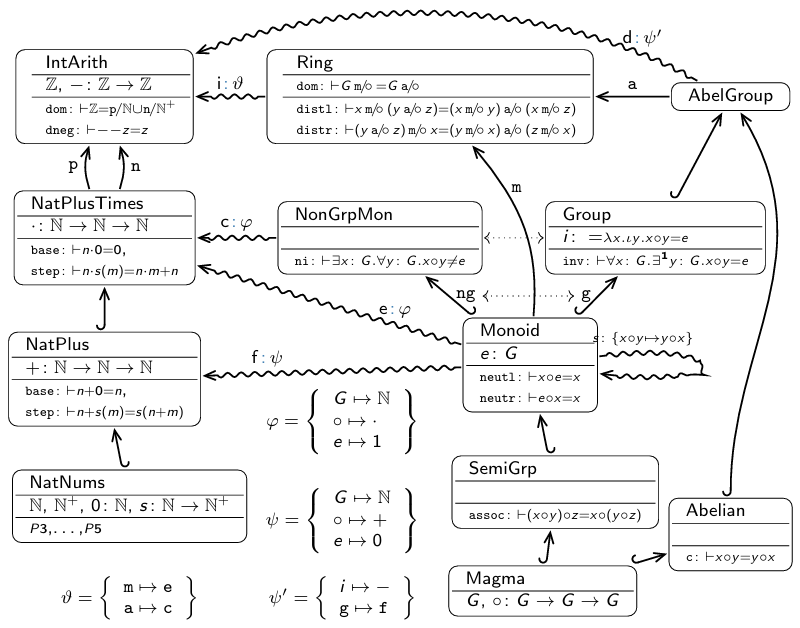
\includegraphics[width=0.7 \linewidth]{images/structures.png}
    \end{center}
\end{figure}
\begin{itemize}
\item nodes are \linkterm{structures}{def:math_structure} with \linkterm{objects}{math_object} ($\circ : \tau$) and properties ($n :\vdash P$).
\item edges represent inheritance
\begin{itemize}
    \item regular inheritance:  $\hookrightarrow$
    \item copying substructures: $\xrightarrow{n}$ 
    \item interpretation via $\varphi$: $\overset{n}{\leadsto}$
\end{itemize} 
\item Examples are just interpretations ($\leadsto$) read backwards
\item Any \linkterm{object}{math_object} / property / \linkterm{theorem}{theorem} can be copied along any edge
\end{itemize}